Як уже згадувалось, домінуючим парамагнітним дефектом зі значенням \mbox{g-фактора} поблизу 2 у кристалах 3C-SiC, опромінених нейтронами, є від'ємнозаряджена вакансія кремнія, центр Т1 \citep{t1}. Спостереження інших парамагнітних дефектів у даному діапазоні \mbox{g-факторів} ускладнюється за рахунок високої інтентивності ліній вищезгаданого спектра. Проте, як видно з рис. 1, відпал при Т\textsubscript{відп}~=~800~$\degree$C призводить до зникнення вакансій кремнія. Унаслідок чтого, як видно з рисунка, з'являється можливість спостереження нового центра, назвемо його Ку6.\\
\\
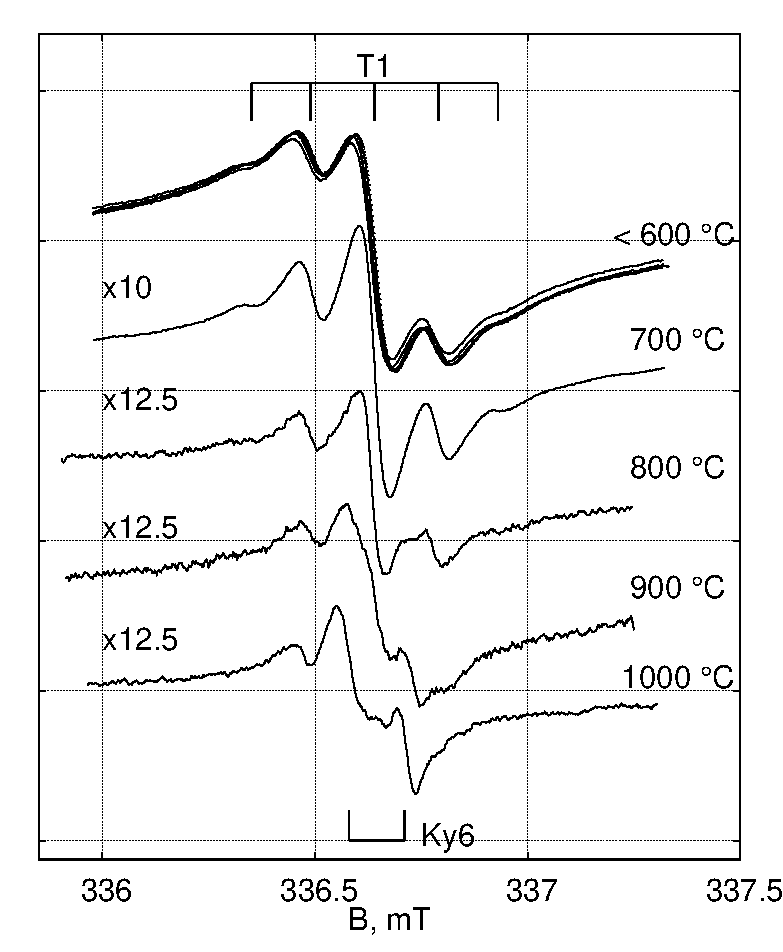
\includegraphics[width=200pt]{images/g1.eps}\mbox{}\\
\small Рис. 1. Кінетика відпалу центра V\textsubscript{Si}\textsuperscript{-} та спостереження ліній ЕПР нового центра Ку6. f~=~9.347~ГГц, B~||~<110>.\\
\\
\normalsize
\indentОкрім того, з рис. 1 видно, що кінетика відпалу від'ємної вакансії кремнія у кристалах, опромінених електронами та нейтронами, має суттєві відмінності. А саме, у той час коли у електронноопромінених кристалах спостерігається 3 стадії відпалу при температурах, відповідно, 150~$\degree$C, 350~$\degree$C та 750~$\degree$C \citep{t1}, для нейтронноопромінених зразків характерна лише одна стадія, яка припадає на температуру 800~$\degree$C та пов'язана з відпалом близько 90\% вихідної концентрації дефекта, що вказує на відмінності у складі системи дефектів, утворених унаслідок опромінення різними типами частинок. Необхідно згадати, що перші дві стадії відпалу центра Т1, пов'язувались із його взаємодією з міжвузловими атомами \citep{t1}. Відсутність цих стадій у зразках, опромінених нейтронами, свідчить про відмінності у положеннях енергетичних рівнів міжвузлових атомів у кристалах, опромінених електронами та нейтронами відповідно.\\
\indentУ зразках, відпалених при Т\textsubscript{відп}~=~800~$\degree$C спектр центра Т1 не спостерігається, проте при температурах нижчих за Т~=~140~К спостерігаються лінії, які належать новому парамагнітному центру Ку6. Кутова залежність ліній ЕПР даного центра (Рис.~2) вказує на його безпосередній зв'язок з дефектом з ефективним спіном S~=~1/2. Параметри спінового Гамільтоніана центра Ку6, визначені з кутової залежності становлять, відповідно, g$_\parallel$~=~2.0024~$\pm$~0.0001 та g$_\perp$~=~2.0039~$\pm$~0.0001, напрямок головної осі \mbox{g-тензора} відповідає вектору <111>. У той же час, теоретичний розрахунок залежності положень резонансних ліній від орієнтації магнітного поля, з урахуванням цих параметрів, свідчить про те, що центр Ку6 добре узгоджується з моделлю з симетрією С\textsubscript{3v}.\\
\\
\includegraphics[width=200pt]{images/g2.eps}\mbox{}\\
\small Рис. 2. Кутова залежність ліній ЕПР центра Ку6. Кругами позначено теоретично розраховані положення ліній. Кут $\theta$ відповідає кристалічним напрямкам 0~$\degree$C~$\equiv$~<001> та 90~$\degree$C~$\equiv$~<110>, відповідно.\\
\\
\normalsize
\indentУ низькопольовій та високопольовій областях спектра ЕПР центра Ку6 спостерігаються чіткі лінії надтонкої взаємодії. Аналіз кутової залежності даних ліній (Рис.~3) свідчить про аксіальність НТВ та дає змогу визначити її параметри. А саме, А$_\parallel$~=~23.9$\cdot$10$^{-4}$~см$^{-1}$ та А$_\perp$~=~19.3$\cdot$10$^{-4}$~см$^{-1}$ та напрямок головної осі тензора уздовж кристалічного напрямку <111>.\\
\\
\includegraphics[width=200pt]{images/g3.eps}\mbox{}\\
\small Рис. 3. Кутова залежність ліній НТВ (квадратами позначено теоретично змодельовані положення ліній). T\textsubscript{відп.}~=~1000~$\degree$C, f~=~9.264~ГГц, Т~=~80~К, B~$\parallel$~(110).\\
\\
\normalsize
\indentІнтенсивність ліній НТВ виявляється достатньою для аналізу природи ядер, з якими вона пов'язана. Після відокремлення корисного сигналу від фонової лінії та шумової доріжки, було отримано значення відношення інтенсивності ліній НТВ до центральних ліній. У даному випадку воно становить 0.13~$\pm$~0.02. Така величина найкраще узгоджується з взаємодією з трьома ядрами кремнію \textsuperscript{29}Si, природна розповсюдженість яких складає відповідно 4.2\%. Таким чином, можна стверджувати, що спінова густина неспарених електронів зосереджена на трьох ядрах кремнію і дефект займає позицію у вузлі ґратки атома вуглецю, який має три атоми кремнія у першій сфері оточення.\\
\indentФакт участі у НТВ лише трьох ізотопів кремнію вказує на комплексну природу дефекту і присутність у одному із вузлів ґратки першої сфери оточення вакансії вуглецю, заміть атома кремнвю, іншої складової цього комплексу. Проте, у такому разі, повинна була б спостерігатись НТВ із ядром іншої складової дефекта, яка, нажаль, спостережена не була. Одним із ймовірних пояснень даного факту може бути присутність у складі комплексу атома вуглецю, магнітний ізотоп якого \textsuperscript{13}С має природну розповсюдженність лише 1.2\%, внаслідок чого роздільної здатності спектрометра може бути не достатньо для його спостереження.\\
\indentОтримані з експерименту параметри дають підґрунтя для побудови впевненої моделі спостереженого центра. Насамперед, з теоретичних робіт \citep{met1,met2,met3,met4} відомо, що для вакасії кремнія V\textsubscript{Si} повинно спостерігатися явище метастабільності. Дане явище пов'язане з достатньо невисоким потенціальним бар'єром для перетворенння вакансії кремнія V\textsubscript{Si} на комплексний дефект вакансія вуглецю - антисайт вуглецю [V\textsubscript{C}C\textsubscript{Si}] (Рис. 4). У 3C-SiC даний бар'єр складає близько 1.9~..~2.5~eV, що для випадку зразків p-типу менше потенціального бар'єру, який необхідно подолати міжвузловим атомам кремнію, для того, щоб анілігювати з вакансією, унаслідок чого такий процес є домінуючим.\\
\\
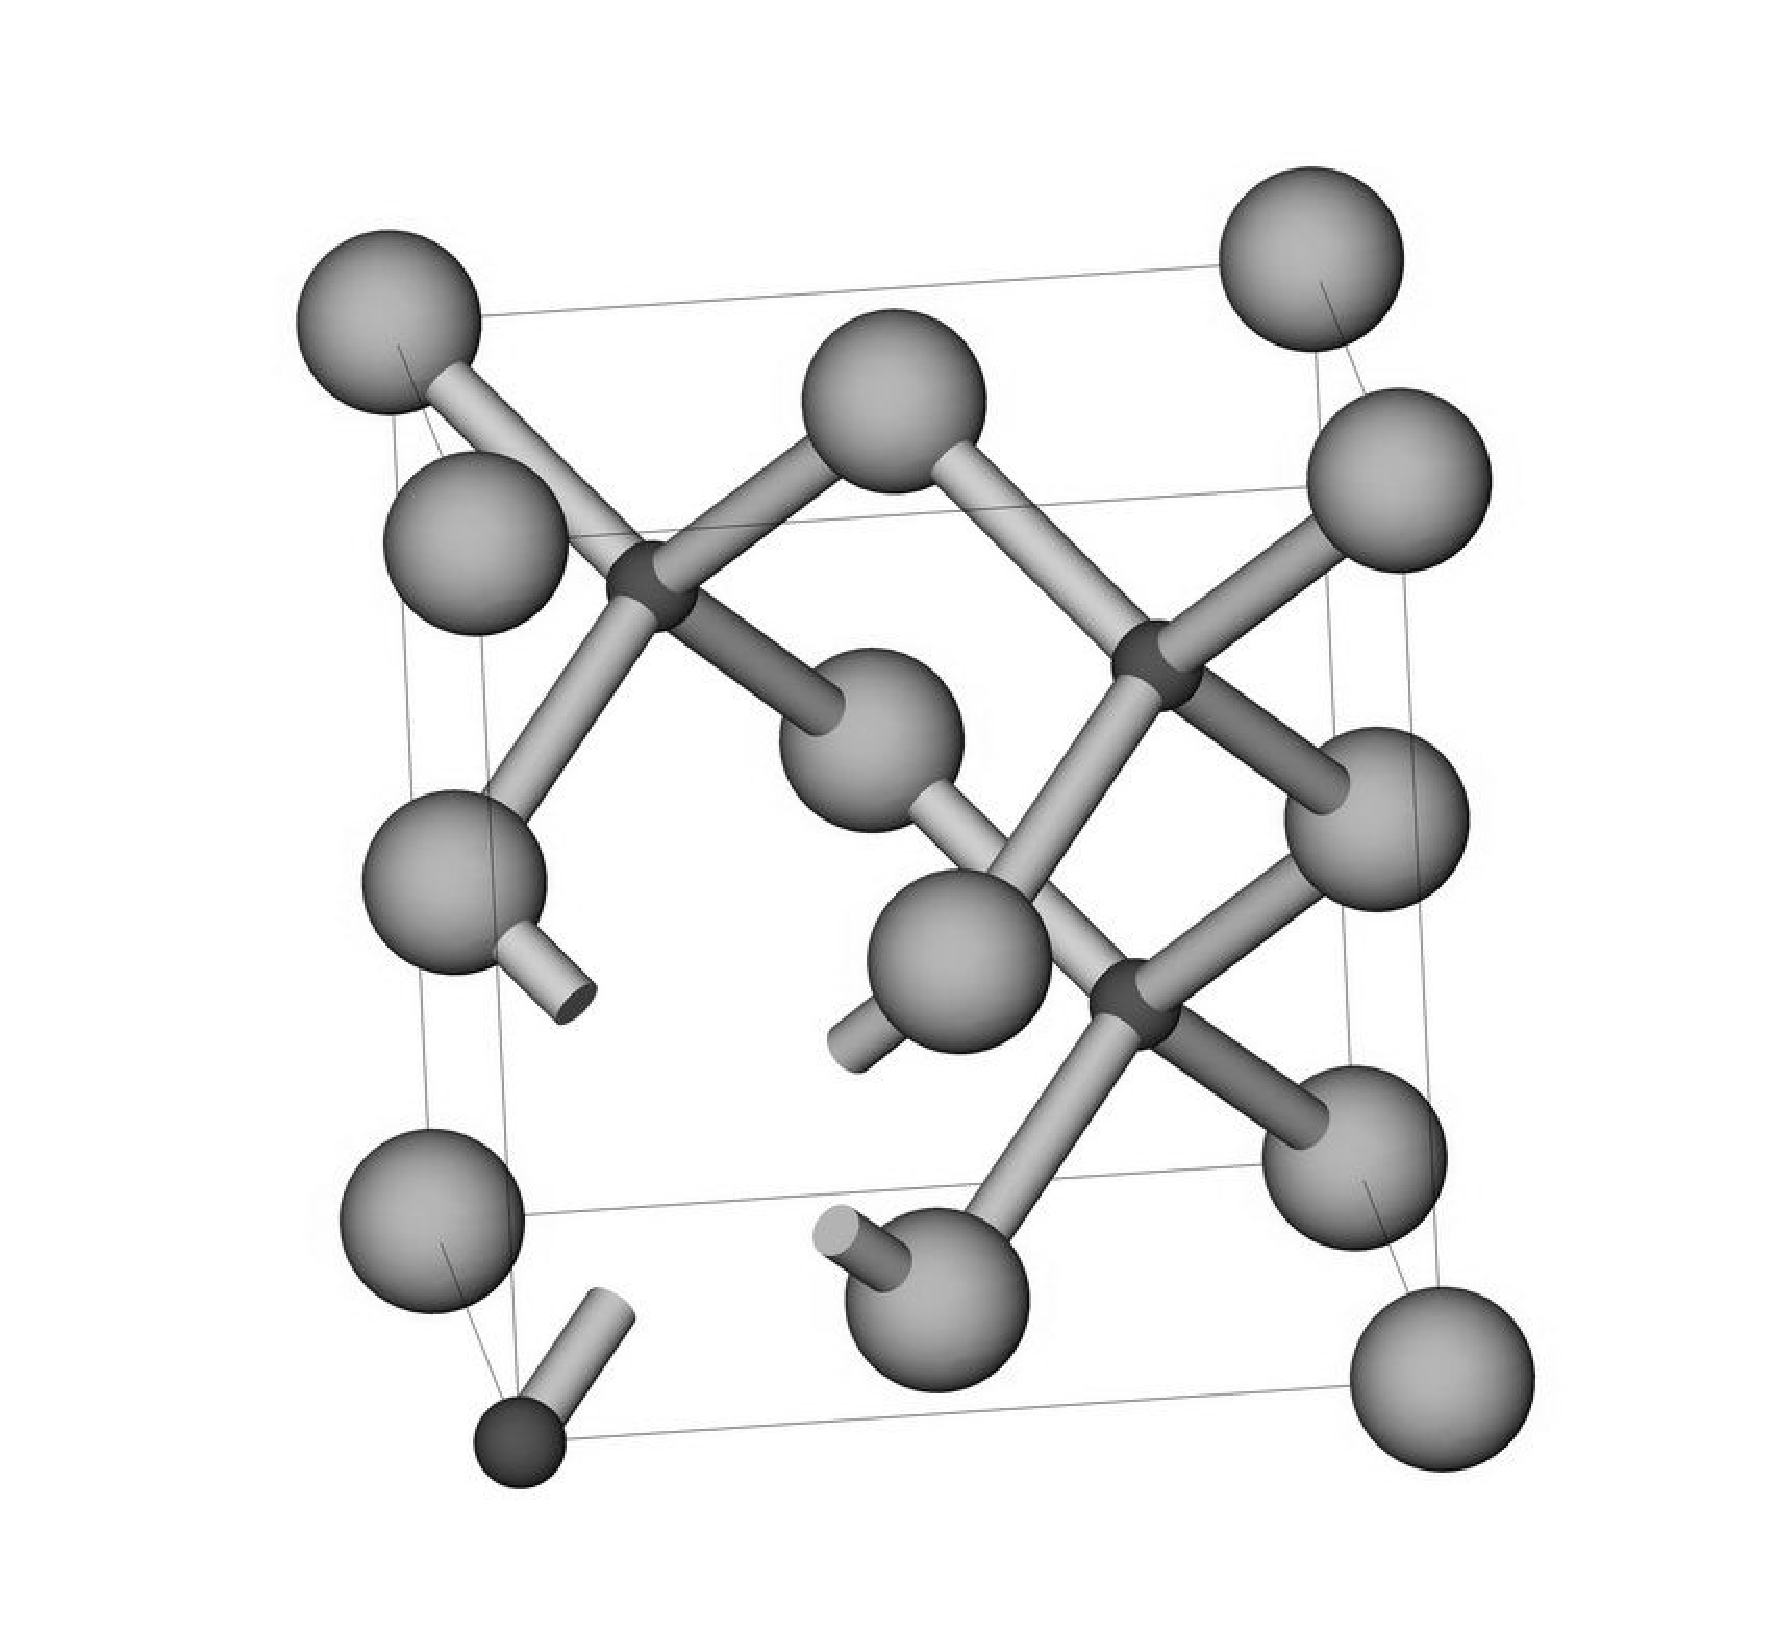
\includegraphics[width=200pt]{images/g4.eps}\mbox{}\\
\small Рис. 4. Атомна модель центра Ку6 [V\textsubscript{C}C\textsubscript{Si}].\\
\\
\normalsize
\indentДля випадку зразків n-типу характерні менші потенціальні бар'єри для міжвузлових атомів, з чим саме і пов'язувались перші дві стадії відпалу V\textsubscript{Si}\textsuperscript{-} у кристалах опромінених електронами \citep{t1}. Проте відпал при температурі близько Т\textsubscript{відп}~=~800~$\degree$C надає кристалу енергію активації 2.2~eV \citep{t1}, яка за величиною відповідає енергії наведеного вище перетворення, у результаті чого дана стадія відпалу повинна бути пов'язана з утворенням комплексу [V\textsubscript{C}C\textsubscript{Si}]. Проте у кубічних кристалах даний дефект раніше не спостерігався.\\
\indentТеотеричні розрахунки енергетични рівнів дефектів для різних зарядових станів,  проведені А.~Маттаушем \citep{met1,met2} свідчать про те, що для положення рівня Фермі, при якому вакансія кремнія існує у 1- зарядовому стані, зарядовий стан комплексу [V\textsubscript{C}C\textsubscript{Si}] повинен бути нейтральним і, у результаті чого, процес зворотньго перетворення має енергію активації 4~eV, що унеможливлює його при даних умовах. Таким чином, враховуючи наведені вище, теоретично розраховані, енергії, кінетику відпалу та результати аналізу спектрів ЕПР, насамперед його НТВ, центр Ку6 ми пов'язуємо з нейтральним комплексом вакансія вуглецю - міжвузля вуглецю [V\textsubscript{C}C\textsubscript{Si}]\textsuperscript{0}.\\
